% Created 2010-10-12 Tue 16:22
\documentclass[presentation]{beamer}
\usepackage[latin1]{inputenc}
\usepackage[T1]{fontenc}
\usepackage{fixltx2e}
\usepackage{graphicx}
\usepackage{longtable}
\usepackage{float}
\usepackage{wrapfig}
\usepackage{soul}
\usepackage{t1enc}
\usepackage{textcomp}
\usepackage{marvosym}
\usepackage{wasysym}
\usepackage{latexsym}
\usepackage{amssymb}
\usepackage{hyperref}
\tolerance=1000
\usepackage[english]{babel} \usepackage{ae,aecompl}
\usepackage{mathpazo,courier,euler} \usepackage[scaled=.95]{helvet}
\usepackage{listings}
\lstset{language=Python, basicstyle=\ttfamily\bfseries,
commentstyle=\color{red}\itshape, stringstyle=\color{darkgreen},
showstringspaces=false, keywordstyle=\color{blue}\bfseries}
\providecommand{\alert}[1]{\textbf{#1}}

\title{Other type of plots}
\author{FOSSEE}
\date{}

\usetheme{Warsaw}\usecolortheme{default}\useoutertheme{infolines}\setbeamercovered{transparent}
\begin{document}

\maketitle









\begin{frame}
\frametitle{Outline}
\label{sec-1}

\begin{itemize}
\item Scatter plot
\item Pie chart
\item Bar chart
\item Log-log Plot
\item \texttt{matplotlib} help
\end{itemize}
\end{frame}
\begin{frame}
\frametitle{Exercise 1: Scatter plot}
\label{sec-2}

  Plot a scatter plot showing the percentage profit of Company A from the year 2000
  to 2010. The data for the same is available in the file \texttt{company-a-data.txt}.
\end{frame}
\begin{frame}[fragile]
\frametitle{\texttt{scatter()} function}
\label{sec-3}

\begin{itemize}
\item \emph{Syntax :} scatter(x,y)

\begin{itemize}
\item x, a sequence of data
\item y, a sequence of data, the same length of x
\end{itemize}

\end{itemize}

\begin{verbatim}
   In []: scatter(year, profit)
\end{verbatim}
\end{frame}
\begin{frame}[fragile]
\frametitle{Exercise 2: Scatter plot}
\label{sec-4}

  Plot a scatter plot of the same data in \texttt{company-a-data.txt} with red diamond markers.
\begin{verbatim}
   
\end{verbatim}

  \textbf{Clue} - \emph{try scatter? in your ipython interpreter}
\end{frame}
\begin{frame}
\frametitle{Pie chart}
\label{sec-5}

  Pie chart - a circle graph divided into sectors, illustrating proportion. 
\end{frame}
\begin{frame}[fragile]
\frametitle{Exercise 3: Pie chart}
\label{sec-6}

  Plot a pie chart representing the profit percentage of company A, with the data 
  from the file \texttt{company-a-data.txt}.
\begin{verbatim}
   
\end{verbatim}

  \emph{(we can reuse the data in lists year and profit)}
\end{frame}
\begin{frame}[fragile]
\frametitle{\texttt{pie()} function}
\label{sec-7}

\begin{itemize}
\item \emph{Syntax :} pie(values, labels=labels)

\begin{itemize}
\item values, the data to be plotted
\item labels, the label for each wedge in the pie chart
\end{itemize}

\end{itemize}

\begin{verbatim}
   In []: pie(profit, labels=year)
\end{verbatim}
\end{frame}
\begin{frame}[fragile]
\frametitle{Exercise 4: Pie chart}
\label{sec-8}

  Plot a pie chart with the same data with colors for each wedges as white, red, 
  magenta, yellow, blue, green, cyan, yellow, magenta, and blue.
\begin{verbatim}
   
\end{verbatim}

  \textbf{Clue} - \emph{try pie? in your ipython interpreter}
\end{frame}
\begin{frame}
\frametitle{Bar chart}
\label{sec-9}

  Bar chart - a chart with rectangular bars with lengths proportional 
  to the values that they represent.
\end{frame}
\begin{frame}[fragile]
\frametitle{Exercise 5: Bar chart}
\label{sec-10}

  Plot a bar chart representing the profit percentage of company A, with the data 
  from the file \texttt{company-a-data.txt}.
\begin{verbatim}
   
\end{verbatim}

  \emph{(we can reuse the data in lists year and profit)}
\end{frame}
\begin{frame}[fragile]
\frametitle{\texttt{bar()} function}
\label{sec-11}

\begin{itemize}
\item \emph{Syntax :} bar(x, y)

\begin{itemize}
\item x, a sequence of data
\item y, a sequence of data, the same length of x
\end{itemize}

\end{itemize}

\begin{verbatim}
   In []: bar(year, profit)
\end{verbatim}
\end{frame}
\begin{frame}
\frametitle{Exercise 6: Bar chart}
\label{sec-12}

  Plot a bar chart which is not filled and which is hatched with 
    $45^o$
  slanting lines as shown in the image. The data for the chart may be
  obtained from the file \texttt{company-a-data.txt}.
   \begin{center}
      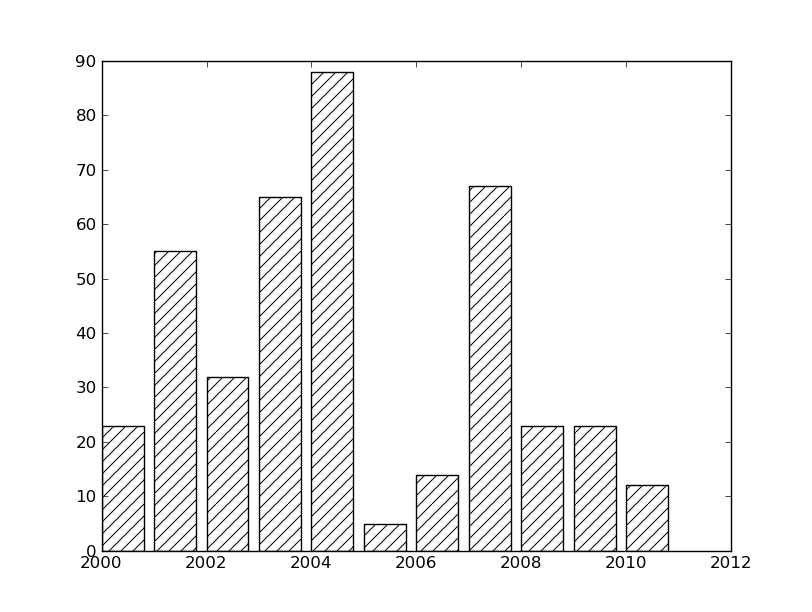
\includegraphics[scale=0.3]{bar-chart-hatch}    
    \end{center}
  \textbf{Clue} - \emph{try bar? in your ipython interpreter}
\end{frame}
\begin{frame}
\frametitle{Log-log graph}
\label{sec-13}

\begin{itemize}
\item Log-log graph

\begin{itemize}
\item 2-dimensional graph.
\item uses logarithmic scales on both axes.
\item graph appears as straight line due to non-linear scaling.
\end{itemize}

\end{itemize}
\end{frame}
\begin{frame}
\frametitle{Exercise 7:}
\label{sec-14}

  Plot a log-log chart of 
    $y = 5x^3$
  for x from 1-20.
\end{frame}
\begin{frame}[fragile]
\frametitle{\texttt{loglog()} function}
\label{sec-15}

\begin{itemize}
\item \emph{Syntax :} loglog(x, y)

\begin{itemize}
\item x, a sequence of data
\item y, a sequence of data, the same length of x
\end{itemize}

\end{itemize}

\begin{verbatim}
   In []: loglog(x, y)
\end{verbatim}
\end{frame}
\begin{frame}
\frametitle{Getting help on \texttt{matplotlib}}
\label{sec-16}

\begin{itemize}
\item Help

\begin{itemize}
\item \hyperref[sec-16]{matplotlib.sourceforge.net/contents.html}
\end{itemize}

\item More plots

\begin{itemize}
\item \hyperref[sec-16]{matplotlib.sourceforge.net/users/screenshots.html}
\item \hyperref[sec-16]{matplotlib.sourceforge.net/gallery.html}
\end{itemize}

\end{itemize}
\end{frame}
\begin{frame}
\frametitle{Summary}
\label{sec-17}

\begin{itemize}
\item Scatter plot (\texttt{scatter()})
\item Pie chart (\texttt{pie()})
\item Bar chart (\texttt{bar()})
\item Log-log plot (\texttt{loglog()})
\item \texttt{matplotlib} online help
\end{itemize}
\end{frame}
\begin{frame}
\frametitle{Thank you!}
\label{sec-18}

  \begin{block}{}
  \begin{center}
  This spoken tutorial has been produced by the
  \textcolor{blue}{FOSSEE} team, which is funded by the 
  \end{center}
  \begin{center}
    \textcolor{blue}{National Mission on Education through \\
      Information \& Communication Technology \\ 
      MHRD, Govt. of India}.
  \end{center}  
  \end{block}
\end{frame}

\end{document}
